\documentclass[11pt]{article}

\usepackage{amsmath}
\usepackage{amssymb}
\usepackage[utf8]{inputenc}
%\usepackage[latin1]{inputenc}
\usepackage[spanish]{babel}
\usepackage[left=3cm,right=3cm,top=3cm,bottom=2.5cm]{geometry}
\usepackage{amsmath,amssymb,latexsym,color,graphicx,verbatim}
\usepackage{mathrsfs}
\usepackage{layout}
\usepackage{graphicx}
\usepackage{multirow}
\usepackage[table,xcdraw]{xcolor}
\usepackage{amsmath} % or simply amstext
\newcommand{\angstrom}{\textup{\AA}}
%COLOCA COMANDOS EN ESPAÑOL
%\renewcommand{\contentsname}{Contenido}
%\renewcommand{\partname}{Parte}
%\renewcommand{\appendixname}{Apéndice}
%\renewcommand{\figurename}{Figura}
%\renewcommand{\tablename}{Tabla}
%\renewcommand{\abstractname}{Resumen}
%\renewcommand{\refname}{Bibliografía}
%FIN DEL BLOQUE
\usepackage[acronym,shortcuts]{glossaries} %PARA UN GLOSARIO DE ACRÓNIMOS
\makeglossaries
\usepackage[font=small]{caption}
\usepackage[colorlinks = true,
                     linkcolor = blue,
                     citecolor = red,
                     urlcolor = blue]{hyperref}

\baselineskip0.75cm
\parskip0.5cm
\parindent0cm

\begin{document}


\begin{titlepage}
\centering \textbf{{\Large {\sc Estudio del último eclipse cromosférico de $\zeta$  Aurigae, otoño 2019}}}

\vfill
\centering {\Large Propuesta de trabajo de grado para optar al t\'itulo de F\'isica}
\vfill
\hfill

\centering {\textbf{\Large Natalia Lucía Oliveros Gómez$^{1,2}$}}

\vfill

\centering {\Large Director: Ph.D Klaus-Peter Schröder $^{3}$}

\centering {\Large  Co-Director: Ph.D Luis Alberto Núñez$^{1,2}$}

\centering {\Large  Co-Director: M.Sc Faiber Danilo Rosas$^{3}$}


\hfill




{{\Large $^1$Grupo de Investigaci\'on en Relatividad y Gravitaci\'on GIRG}} \\
{{\Large$^2$Grupo Halley de Astronom\'ia y Ciencias Aeroespaciales}} \\
{{\Large$^3$Grupo de Investigación en Física Estelar, Universidad de Guanajuato}} \\

\vfill
\vfill

\centering {\Large Universidad Industrial de Santander\\Facultad de
Ciencias\\Escuela de F\'{i}sica\\Bucaramanga\\2020}


\end{titlepage}


\newpage

\tableofcontents

%\newpage

%\acrodef{LAGO}{Latin American Giant Observatory}

\newpage




%%%%%%%%%%%%%%%%%%%%%%%%%%%%%%%%%%%%%%%%%%%%%%%%%%%%%%%%%%%%%%%%%%%%%%%%%%%%%%%%%%%%%%%%%%%%%%

\begin{table}[htbp]
\begin{center}
\resizebox{14cm}{!}{
\begin{tabular}{|l|l|l|l|l|}
\hline
\multicolumn{5}{|l|}{\begin{tabular}[c]{@{}l@{}}\textbf{Título de la propuesta:}\\ Estudio del último eclipse cromosférico de $\zeta$ Aurigae, otoño 2019\end{tabular}}           \\ \hline
\multicolumn{5}{|l|}{\begin{tabular}[c]{@{}l@{}}\textbf{Nombre del estudiante:}\\ Natalia Lucía Oliveros Gómez\end{tabular}}                                                    \\ \hline
\textbf{Código:} 2160778                          & \multicolumn{3}{l|}{\textbf{E-mail:} onatalialucia@gmail.com}                              & \textbf{Cel:} 3123154756                         \\ \hline
\multicolumn{5}{|l|}{\begin{tabular}[c]{@{}l@{}}\textbf{Nombre del grupo de Investigación:}\\ Física Estelar de la Universidad de Guanajuato\end{tabular}}                                           \\ \hline
\multicolumn{5}{|l|}{\begin{tabular}[c]{@{}l@{}}{\textbf{Dirección:} Callejón de Jalisco S/N, Col. Valenciana , CP: 36023\\ Guanajuato, Gto, México. Departamento de Astronomía}                 \end{tabular}}                                                                            \\ \hline
\textbf{Tel:} 1 473 732 0006                                     & \multicolumn{4}{l|}{\textbf{E-mail: } astrokp85@gmail.com}                                                                                                \\ \hline
\multicolumn{5}{|l|}{\begin{tabular}[c]{@{}l@{}}
{\textbf{Líneas de investigación desarrolladas por el grupo:} Atmósferas estelares,\\ evolución estelar, sistemas binarios }\end{tabular}}              \\ \hline
\multicolumn{5}{|l|}{\begin{tabular}[c]{@{}l@{}}\textbf{Profesor de la Escuela de Física que dirigirá el trabajo:}\\ Ph.D Luis Alberto Núñez de Villavicencio Martínez \end{tabular}} \\ \hline
\multicolumn{5}{|l|}{\begin{tabular}[c]{@{}l@{}}\textbf{Profesional del grupo de investigación que servirá de tutor:}\\ Ph.D Klaus-Peter Schröder\end{tabular}}              \\ \hline
\end{tabular}}
\end{center}
\end{table}

\newpage
%%%%%%%%%%%%%%%%%%%%%%%%%%%%%%%%%%%%%%%%%%%%%%%%%%%%%%%%%%%%%%%%%%%%%%%%%%%%%%%%%%%%%%%%%%%%%%
\begin{abstract}
En el presente proyecto se realiza un análisis de la variación de la densidad de masa columnar en la cromosfera de la estrella $\zeta$ Aurigae durante su último eclipse en otoño de 2019. Se hace un estudio de la variabilidad temporal de la línea de calcio ionizado K de CaII (3934 $\angstrom$), usando espectros con relación S/N de 200-300 y resolución de $\sim$ 20000 obtenidos por TIGRE-HEROS. Teniendo en cuenta datos de eclipses anteriores para el mismo sistema y resultados de este proyecto, se busca proponer un modelo que explique el cambio de densidad de masa columnar con la altura en la cromosfera de la estrella gigante y la dinámica del sistema.

\vspace{0.5cm}
\textbf{Palabras clave:} Estrellas binarias eclipsantes, cromosfera estelar, curvas de crecimiento, espectroscopia.

\end{abstract}


\begin{figure}
  \centering

  \label{Figura 1}
\end{figure}


\section{Grupo de Investigación de la Universidad de Guanajuato}

El grupo de investigación de \textit{Física Estelar}, al cual pertenece el Ph.D Klaus-Peter Schröder y el MSc. Faiber Rosas, tiene como objetivo el estudio del nacimiento, la evolución y la muerte de las estrellas frías y las estrellas masivas.  Los proyectos e investigaciones se hacen aplicando los principios de la física para modelar el interior de la estrella, su atmósfera y su viento, así como las interacciones en sistemas estelares binarios y en sistemas planetarios. Además del uso modelos teóricos para explicar fenómenos físicos, también se analizan datos observacionales del telescopio TIGRE  \footnote{El telescopio TIGRE es una de las herramientas por las cuales se tiene una un convenio bilateral entre la Universidad de Guanajuato - México, la Universidad de Hamburgo - Alemania y la Universidad de Liège - Bélgica.} \cite{schmitt2014tigre}, para obtener propiedades intrínsecas de estrellas frías.

\noindent De manera más específica, para estrellas masivas, la investigación se centra en la estructura de los vientos estelares, modelar efectos de rotación,  inestabilidades intrínsecas, interacciones en sistemas binarios y evolución estelar. Se busca determinar con precisión parámetros principales como temperatura efectiva, gravedad superficial y composición química, con el uso de modelos fotosféricos generados con el código PHOENIX  \footnote{Código que permite modelar atmósferas estelares y espectros teóricos de diferentes tipos de estrellas.} \cite{hauschildt2005cool} y análisis de espectros del telescopio TIGRE. Al implementar tanto simulaciones como análisis de datos observacionales, se puede comprender aún mejor la actividad y evolución de estrellas como el Sol, que en el caso en que solo se usara uno de estos métodos. Para el caso de estrellas jóvenes, la investigación tiene un enfoque en el cálculo de la emisión de polvo en sistemas circumplanetarios que las rodean; esto permite caracterizar la distribución de material en los discos, que a su vez tiene que ver con la presencia de planetas. 

\section{Lugar dentro de los proyectos del grupo de investigación}
\noindent Este proyecto se realizará en el marco de pasantía de investigación y está enfocado en el área de interacción de sistemas estelares binarios, ya que se hará un análisis de espectros tomados por el telescopio TIGRE, los cuales cambian en el proceso de interacción de atmósferas durante el eclipse del sistema Zeta Aurigae. Otra de las áreas que se aborda es atmósferas estelares, ya que se analizará la cromosfera de la estrella gigante fría del sistema, implementando códigos de simulación para este tipo de estrellas. También se tendrá en cuenta parámetros principales que necesitan alta precisión como: temperatura efectiva, gravedad superficial y composición química. El sistema binario antes mencionado fue estudiado por el profesor Klaus-Peter Schröder en los años 80 \cite{kps9}, \cite{kps1O}, por lo tanto, con la experiencia en dicho sistema, resulta relevante retomar estos estudios, ya que en la actualidad se tiene más conocimiento en el área y mejores tecnologías que en aquella época, lo cual permite desarrollar análisis más concretos.

\section{Problema de investigación}

\noindent Los sistemas de estrellas binarias eclipsantes están formados por dos estrellas cuyo plano orbital está orientado hacía la Tierra. Por lo tanto, cuando se miden espectros de estos sistemas, en el transcurso del eclipse las componentes espectrales de cada estrella se superponen, haciendo que los espectros individuales no puedan ser reconocibles. Sin embargo, se puede hacer una sustracción espectral para cada estrella si se tienen espectros de la estrella principal sin eclipsar y así comparar con los espectros durante el eclipse. Cuando se logra la separación de espectros en sistemas binarios son una herramienta de los astrónomos para obtener información de cantidades físicas fundamentales de las estrellas, como radios estelares, velocidades orbitales, masas de manera muy precisa, consideraciones geométricas del eclipse y temperaturas efectivas \cite{schroder2009stars}.


\noindent En el transcurso del tiempo se han hecho análisis de sistemas binarios eclipsantes, en especial donde una de las componentes estelares es una estrella gigante fría. Además, estas estrellas nos permiten obtener información para conocer de manera más clara los fenómenos físicos que ocurren en la cromosfera de las estrellas. Cuando la estrella compañera se aproxima a la estrella gigante roja, en los espectros debido al eclipse se pueden apreciar líneas de absorción adicionales que revelan cambios en temperatura, densidad, extensión y movimiento de la cromosfera, que es la región estelar de transición turbulenta entre la fotosfera (superficie de la estrella) y la corona (donde se transporta y pierde materia por vientos solares). Los datos obtenidos en el proceso del eclipse son de alta relevancia en la física estelar ya que con los sistemas binarios se obtiene una forma de medir la masa estelar directamente con el uso de las leyes de Kepler y por ende se pueden calibrar trayectorias estelares evolutivas con mayor precisión. 

\noindent El sistema binario a analizar en este proyecto es Zeta Aurigae, el cual está compuesto por $\zeta$ Aur A, una supergigante roja de tipo espectral K5II; y $\zeta$ Aur B una estrella de la secuencia principal de tipo espectral B7V \cite{shenavrin2011vizier}. Éste sistema se encuentra ubicado en la constelación de Auriga  y en él se presenta el fenómeno de eclipses atmosféricos, los cuales se pueden observar a simple vista, ya que durante los eclipses la magnitud de $\zeta$ Aur A disminuye a +3,99 en la banda V. Este sistema resulta relevante, ya que hasta el momento no ha sido muy analizado y no se tienen muchos datos observacionales del mismo.
\vspace{2mm}

\noindent En trabajos anteriores se han hecho análisis de fotometría y espectroscopia de este sistema con el enfoque de observar el cambio de las líneas de absorción durante el eclipse, dando información importante respecto a la geometría del eclipse, velocidades radiales, masa estelar y luminosidad \cite{kps9}. También se han hecho análisis a partir de \textit{curvas de crecimiento experimentales} \cite{complete}, las cuales son gráficos del ancho equivalente de la línea ($log(W_{\lambda})$) se relaciona con la profundidad de la línea en el espectro ($log(\tau)$) que se refiere a la fuerza de la línea en el espectro. Estas curvas se hacen teniendo en cuenta modelos de densidad e intentando analizar la estructura cromosférica partiendo de la ionización, turbulencia y cambios en la temperatura efectiva. Sin embargo, aún no hay conclusiones específicas de lo que pasa en la atmósfera estelar respecto al cambio en la densidad de masa columnar de átomos del elemento analizado en la fotosfera y cromosfera a medida que cambia la altura, es decir, cambio en la densidad de átomos de H por área por camino óptico entre la estrella y el observador \cite{rybicki2008radiative}. Inicialmente en los espectros se observaba que todas las líneas metálicas tienen el mismo comportamiento, es decir, que la ionización no cambia con respecto a la altura de la atmósfera, donde para bajas alturas la ionización de los metales es casi completa. Pero en el caso de  las líneas de absorción de H y Ca II K (que son las líneas más afectadas durante los eclipses) cambia la ionización media rápidamente con la altura en un factor de 100 con respecto a los demás metales, es decir, que las líneas de Ca II K son un caso anómalo en los eclipses y no se conoce la razón física de que esto suceda \cite{complete}.

\noindent De acuerdo a los trabajos citados anteriormente, surge la necesidad de hacer un análisis que verifique investigaciones de hace más de 30 años, desde un enfoque espectroscópico de la densidad de columna cromosférica, la cual tiene una dependencia con la altitud del eclipse. Y de esta forma intentar aclarar fenómenos que antes no podían ser explicados con los modelos de la época según las observaciones espectroscópicas, como por ejemplo la dinámica envuelta en la cromosfera por medio de perfiles de densidad. 

\noindent Es muy importante en este planteamiento el uso de espectroscopia, ya que las líneas de absorción varían con la densidad. En la parte alta se observan algunas líneas fuertes y en la parte baja de la atmósfera hay muchas líneas débiles. En el caso de espectros puros se pueden medir mientras no esté eclipsado, con las líneas H y K de Ca II (396,847 nm y 393,368 nm) de la fotosfera que son bastante anchas y se comprueba la emisión central de la estrella gigante, estas líneas estándar tienen características de tipo tardío, ya que es una estrella K y se puede definir una escala $\lambda$. También se pueden medir mediante perfiles de dispersión. Para los espectros compuestos, es decir durante el eclipse, se observan cambios en el espectro, estos son de dispersión media y se observan como ``ruido'' en la contribución al espectro puro de la gigante donde las líneas K desvanecen y se observa que por la presencia de la estrella B7 se tienen líneas anchas e intensas de Ca II que cambian su ancho y fuerza durante el eclipse y no es fácil de hacer una distinción de componentes estelares; además no es posible saber cómo hacer la sustracción de espectros para obtener el de la estrella B. En el eclipse total hay una fuerte absorción mayor de Ca II K y por ende más cantidad de líneas de absorción cromosférica, y es la oportunidad de hacer la sustracción de los espectros de la gigante para hacer las respectivas curvas de crecimiento experimentales. 



%%%%%%%%%%%%%%%%%%%%%%%%%%%%%%%%%%%%%%%%%%%%%%%%%%%%%%%%%%%%%%%%%%%%%%%%%%%%%%%%%%%%%%%%%%%%%%
\section{Justificación}

\vspace{3mm}

Durante el siglo pasado la visión de la astronomía pasó de ser una ciencia puramente observacional basada en modelos empíricos a una en donde los fundamentos no solo son experimentales sino también teóricos por medio de principios físicos, dando así paso a la actual astrofísica. Dicha revolución permitió usar el universo como un enorme laboratorio natural, en el que podemos probar nuestras teorías físicas en condiciones extremas (temperaturas altas o bajas, densidades, presiones), que no podemos realizar y probar en laboratorios artificiales. De esta manera, la astronomía y la astrofísica se ha convertido en un campo muy importante de la física.

Para realizar el análisis cromosférico de este sistema binario, a pesar de que es un tema del área de la astronomía, es natural conocer la estrecha relación que tiene esta rama con la física, por lo tanto aunque desde la UIS no se trabaje explícitamente en astronomía o al menos no en análisis de datos observacionales es imprescindible aplicar conceptos físicos, lo cual certifica las competencias como física en la universidad. Dentro de los conceptos físicos empleados en el estudio de sistemas binarios está la espectroscopia, donde es muy importante conocer la interacción fotón-átomo que incluye tipos de absorción, dispersión de resonancia, emisión (re-emisión). También la transferencia radiativa es indispensable al observar el proceso durante el paso de la radiación por la atmósfera de una estrella; adicionalmente cabe resaltar el papel de la teoría atómica al analizar los cambios en la atmósfera estelar (por procesos de ionización y demás). 

\begin{comment}
Es necesario recordar que en este caso para el sistema de Zeta Aurigae no resultan relevantes los efectos relativistas ya que no se trata de un sistema binario en el que las estrellas estén muy próximas (4,2 UA) \cite{kps9} y estén interactuando más allá de la gravitación que las mantiene en órbita, no está cambiando la métrica ni otros aspectos en lo que la perturbación relativista sea relevante, por lo tanto se analiza la dinámica de este sistema como un problema clásico.
\end{comment}

Por otro parte, desde la rama observacional, dos características fundamentales para la detección y el estudio de sistemas de estrellas binario son el brillo y el periodo. El primero se relaciona con la capacidad de detección por astrónomos observacionales mientras que el segundo es inversamente proporcional a la cantidad de datos, ya que normalmente los estudios de observación requieren de tiempo en observatorios para poder hacer relaciones y comparaciones temporales. En estos sistemas la relación más óptima son altos brillos y bajos periodos. Sin embargo Zeta Aurigae aunque tiene un alto brillo, también tiene un alto periodo (972 días) \cite{wright1970zeta} de tal manera no se tienen muchos datos al respecto, por lo que se ha dificultado su estudio, haciendo que actualmente exista una brecha entre la literatura de $\aprox$ 30 años  \cite{kps9}, \cite{kps1O}, \cite{complete}, \cite{eaton1993chromospheric}. Debido a esto, resulta importante retomar o tener en cuenta algunos de los resultados que se han obtenido y verificarlos para presentar mejoras o aportes a algunos desarrollos respecto a este sistema binario, como en el caso de la densidad columnar. Cabe resaltar que debido a distancia entre las estrellas del sistema binario (4,2 UA) \cite{kps9} los efectos relativistas no toman relevancia y este se puede tratar como un sistema clásico.

%En este párrafo lo que quiero expresar, es la conexion que existe entre los modelos de la cromosfera viejos y los datos observaciones viejos, y como vos vas a intentar unir esos modelos con los nuevos datos y solucionar discrepancias.

Debido a la ausencia de nuevos datos observacionales, solo se tienen modelos fenomenológicos propuestos para el sistema \cite{kps9} y  análisis de la atmósfera estelar \cite{kps1O}, \cite{complete} en el que se consideran leyes de decaimiento exponencial (\ref{eq:leybaro}) para relacionar escalas de densidad columnar y altura. 

\begin{equation}
    n(h) = n_o \exp{(-h/\alpha)}
    \label{eq:leybaro}
\end{equation}

Sin embargo debido a las recientes medidas del telescopio el TIGRE  eclipse de otoño del 2019 con mejor resolución espectral $\sim 20000$ y relación S/N 200-300, se han observado variaciones de densidad no uniforme respecto a la ionización de metales y con estas variaciones se pueden afectar posibles conclusiones de la dinámica de la cromosfera de las estrellas, incluyendo la geometría del eclipse, masa estelar, luminosidad, velocidad radial, temperatura efectiva y densidad columnar. Motivados por esto resulta relevante verificar lo que se ha concluido hasta el momento y si es necesario proponer otro modelo de densidad que se ajuste mejor a los parámetros geométricos del eclipse y que tenga en cuenta dichas variaciones como el caso de ionización de elementos en la atmósfera, reduciendo así las incertidumbres.

\begin{comment}
se observa que las variaciones de la densidad de columna puede no estar siguiendo el mismo modelo que se había considerado, ya que los cambios que se estaban considerando como constantes pueden realmente afectar posibles conclusiones de la dinámica de la cromosfera de las estrellas.

Por lo tanto algunas de estas suposiciones y conclusiones a las cuales se han llegado no son suficientes para llegar hipótesis relevantes que expliquen la dinámica de la cromosfera.

Gracias a las nuevas observaciones realizadas por TIGRE, con estos datos se puede analizar y conocer la dinámica del sistema como lo son la geometría del eclipse, masa estelar, luminosidad, velocidad radial, temperatura efectiva y densidad de columna, los cuales están englobados al hacer un análisis de la cromosfera de la estrella gigante pura con respecto a las variaciones de la misma en el transcurso del eclipse.
\end{comment}

\begin{comment}
En el siglo pasado, se consideraba que la astronomía tenía un carácter de una ciencia puramente observacional y empírica, sin embargo en la actualidad, se ha confirmado que no basta solo con modelos empíricos, sino que es necesario que estos estén sustentados física y matemáticamente, por lo tanto es lo que ahora se ha convertido en ``Astrofísica'': la aplicación de la física a los objetos astronómicos. En este sentido, utilizamos el universo como un enorme laboratorio natural, en el que podemos probar nuestras teorías físicas en condiciones extremas (temperaturas altas o bajas, densidades, presiones), que no podemos realizar y probar en laboratorios artificiales. De esta manera, la astronomía y la astrofísica se ha convertido en un campo muy importante de la física.
\end{comment}


\noindent Adicionalmente debido a mi aspiración en hacer una maestría en astronomía es muy importante tener la oportunidad de trabajar con datos reales de un observatorio astronómico internacional, además de datos del repositorio Gaia de la ESA \cite{carrasco2006diseno}, los cuales son datos de paralaje con mayor precisión actualmente, permitiendo calcular luminosidades estelares muy acertadas \cite{fustes2014extraccion}. Para hacer el análisis de estos datos es necesario tener hacer consideraciones relevantes y aplicar modelos físicos para reducir datos y comprender fenómenos de la física que se encuentran en ellos con el enfoque astronómico de la rama de física estelar.

%%%%%%%%%%%%%%%%%%%%%%%%%%%%%%%%%%%%%%%%%%%%%%%%%%%%%%%%%%%%%%%%%%%%%%%%%%%%%%%%%%%%%%%%%%%%%%
\section{Objetivos}

%%%%%%%%%%%%%%%%%%%%%%%%%%%%%%%%%%%%%%%%%%%%%%%%%%%%%%%%%%%%%%%%%%%%%%%%%%%%%%%%%%%%%%%%%%%%%
\textbf{Objetivo General}

\begin{itemize}
\item Comparar la absorción cromosférica y el cambio de la densidad de columna N(h) del eclipse de otoño 2019 con un antiguo eclipse de 1987.
\end{itemize}
\textbf{Objetivos Espec\'ificos}
\begin{enumerate}
    \item Cuantificar el ancho equivalente las líneas claves (Ca II) de las dos estrellas y la  absorción cromosférica

    \item Realizar un análisis de las curvas de crecimiento observacionales

    \item Deducir la densidad en columna y comparar con los resultados publicados, obtenidos en eclipses pasados
\end{enumerate}

%%%%%%%%%%%%%%%%%%%%%%%%%%%%%%%%%%%%%%%%%%%%%%%%%%%%%%%%%%%%%%%%%%%%%%%%%%%%%%%%%%%%%%%%%%%%%%

\section{Metodolog\'ia}

Para alcanzar el objetivo general, es necesario culminar con los objetivos específicos, por los tanto  se proponen una serie de actividades que están relacionadas con cada uno de los objetivos específicos de acuerdo al número asignado anteriormente:

\begin{itemize}

\item[1.1] Instalar y aprender a usar softwares para análisis de espectros:
\begin{itemize}
    \item iSpec: Genera síntesis espectrales, permite encontrar parámetros estelares mediante ajuste de líneas espectrales y ajuste del continuo usando modelos \cite{blanco2014determining}, \cite{blanco2019modern}.
    \item Código que permite analizar la absorción de la línea K de Ca II, permite medir el ancho de línea y el área bajo la curva
    \item Código de evolución estelar: Genera trayectorias evolutivas para determinar masas y edades de las estrellas en un diagrama HR \cite{pols1998stellar}, \cite{schroder1997critical}.
\end{itemize}
\item[1.2] Clasificar la lineas cromosféricas de la estrella gigante y la secundaria
\item[1.3] Obtener un registro de los espectros en orden temporal y calcular en cada caso la altitud proyectada de la compañera sobre la fotosfera del gigante

\item[1.4]  Usar el espectro puro de la gigante durante la totalidad del eclipse para sustraer los espectros compuestos para obtener y obtener el espectro puro la compañera, en el cual se vean las lineas cromosféricas

\item[1.5] Cuantificar el ancho equivalente de las líneas cromosféricas (área de línea de absorción dividido por el continuo local)

\item[2.1] Graficar curvas de crecimiento para cada sesión del eclipse (estrella individual parcial `tanto entrada como salida' y total). Igualmente para el hidrógeno y para el Ca II 

\item[3.1] Comparar diferentes parámetros (\textit{ionización, temperaturas efectiva, ancho doppler,número de átomos, velocidades radiales}) con la densidades de columna N(h)

\item[3.2] Deducir un sencillo modelo de la densidad de columna en cada caso

 %%%%%%%%%%%%%%%%%%%%%%%%%%%%%%%%%%%%%%%%%%%%%%%%%%%%%%%%%%%%%%%%%%%%%%%%%%%%%%%%%%%%%%%%%%%%%%
\end{itemize}
\begin{comment}
Con estas actividades voy a poder desarrollar ciertas competencias que resultan muy útiles e importantes para trabajos a futuro:

\begin{itemize}
    \item Identificación de líneas espectrales y clasificación de espectros
    \item Uso de gráficas basado en plataformas de linux
    \item Entender y aplicar la física espectroscopia de líneas de absorción
    \item Obtener un fondo de la física de atmósferas estelares
\end{itemize}
\end{comment}


\section{Resultados esperados}

Como resultado principal está identificar las diferencias y/o similitudes entre los análisis realizados del sistema Zeta Aurigae de \cite{kps1O}, \cite{complete} con relación a los datos obtenidos del eclipse de otoño del 2019. Para poder argumentar el comportamiento de los espectros en función del tiempo durante el eclipse. Además de explicar las posibles causas del cambio en las hipótesis sobre la dinámica del sistema durante los últimos 30 años. Teniendo en cuenta que la tecnología desde esa época a la actualidad ha cambiado y las herramientas que se tienen ahora son mucho más eficientes en aspectos técnicos.

\begin{comment}
Cabe resaltar que a medida que ha pasado el tiempo desde los análisis anteriores a la actualidad (aproximadamente 30 años) no ha pasado el tiempo suficiente como para que exista la posibilidad de que hallan cambios debido a la evolución estelar del sistema binario que puedan afectar de manera significativa los resultados obtenidos, por lo tanto sabremos que las condiciones en las que se analizaran son aproximadamente las mismas como para concluir que si hay cambios, estos se han efectuado bajo los mismos parámetros que se habían analizado antes.
\end{comment}


Otro de los resultados es una posible verificación del efecto Wilson-Bappu, correlación entre el ancho medido de la línea Ca II K ($W_0$) que depende de la luminosidad de la estrella y por ende de la gravedad superficial; y de la temperatura efectiva y la magnitud visual absoluta de la estrella ($M_{\nu}$) debido al mecanismo de la física estelar. Este efecto se analizó para el sistema $\zeta$ Aurigae en \cite{Dani} donde se observa que en el análisis de espectros con el ensanchamiento de líneas se está verificando el cambio en la gravedad superficial. Teniendo en cuenta que la densidad de masa columnar y la gravedad superficial, tienen una relación inversamente proporcional, indirectamente se esta relacionando el cambio espectral con el objetivo principal del proyecto, así que con ayuda de las curvas de crecimiento y un análisis profundo de los efectos físicos que se están presentando en este sistema, se puede verificar esta relación entre estas cantidades físicas.

\noindent Los resultados mencionados anteriormente son relevantes en el ámbito de la astronomía ya que al conocer la dinámica cromosférica, ya sea de una o un sistema de estrellas, es posible tener mayor precisión de sus parámetros físicos relevantes y esto a su vez aporta correcciones a las curvas estelares evolutivas \cite{pols1998stellar}.  

Por último es importante la experiencia que se adquiere durante este proceso en el área de la física, aportando a su vez hacía la formación futura como astrofísica, además también me permite hacer parte de una colaboración internacional para escribir un artículo científico en una revista arbitrada donde se vean reflejados los resultados más importantes que se obtengan del sistema Zeta Aurigae.



%%%%%%%%%%%%%%%%%%%%%%%%%%%%%%%%%%%%%%%%%%%%%%%%%%%%%%%%%%%%%%%%%%%%%%%%%%%%%%%%%%%%%%%%%%%%%%

\section{Condiciones y recursos que ofrece el grupo de investigación}

El grupo de investigación de Física estelar brinda los datos que se usarán para resolver este proyecto, los cuales fueron tomados por el telescopio el TIGRE, explicado en sesiones anteriores por el convenio con la Universidad de Hamburgo en Alemania, de la Universidad Liège, en Bélgica, adicional a esto es donde se encuentran los especialistas en el área de astronomía estelar, los cuales han trabajado en años anteriores con este mismo sistema binario en incluyendo algunos de los aspectos que se tendrán en cuenta en este proyecto, por último brindan las instalaciones del grupo en el cual tendré un lugar de trabajo dentro de la Universidad en la estancia de cuatro meses.
%%%%%%%%%%%%%%%%%%%%%%%%%%%%%%%%%%%%%%%%%%%%%%%%%%%%%%%%%%%%%%%%%%%%%%%%%%%%%%%%%%%%%%%%%%%%%%
\vspace{45mm}

\section{Cronograma de Actividades}

\vspace{2mm}

\begin{figure}[h]
    \centering
    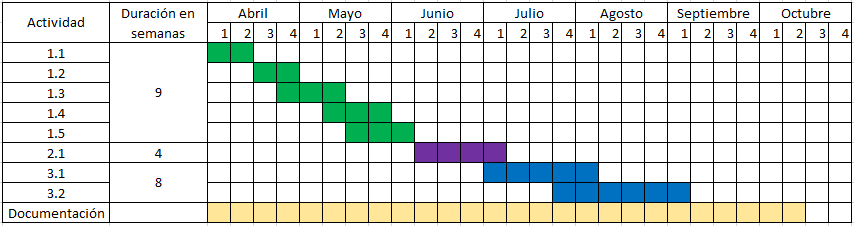
\includegraphics[width=1\linewidth]{Cronograma.PNG}
\label{Cronograma}
\end{figure}

%%%%%%%%%%%%%%%%%%%%%%%%%%%%%%%%%%%%%%%%%%%%%%%%%%%%%%%%%%%%%%%%%%%%%%%%%%%%%%%%%%%%%%%%%%%%%%
\bibliographystyle{unsrt}
\bibliography{BIBLIO.bib}


\section{ Anexos}

Carta de aceptación en el programa de movilidad para el semestre 2020-1.
%%%%%%%%%%%%%%%%%%%%%%%%%%%%%%%%%%%%%%%%%%%%%%%%%%%%%%%%%%%%%%%%%%%%%%%%%%%%%%%%%%%%%%%%%%%%%%

%%%%%%%%%%%%%%%%%%%%%%%%%%%%%%%%%%%%%%%%%%%%%%%%%%%%%%%%%%%%%%%%%%%%%%%%%%%%%%%%%%%%%%%%%%%%%%
\end{document}
